\chapter{Tune for the Primordial $k_T$}
\label{chap:primordialkTtune}

The primordial $k_T$ is another important parameter in the description of the proton-proton collisions with Monte Carlo simulations. The primordial $k_T$ description in \textsc{pythia8} was introduced in \secRef{sec:Beam Beam Remnants and primordial kT}.
\\
The main unresolved problem for the primordial $k_T$ tune is the unexpected high value required for the description of the observed $Z$ boson $p_T$ spectrum.
\\
In fact, the primordial $k_T$ found is origin in the Fermi Motion of the partons inside the hadrons. So when the parton undergoes to the hard scattering it can already have an initial no zero transverse momentum.
The value of the primordial $k_T$ can be estimate as reported in \eqRef{eq:PrimordialKT}, but in the case of the $Z$ boson $p_T$ spectrum this estimation is not sufficient the required value observed in order to reproduce the experimental data are in the order of $2\ \mathrm{GeV}$.

%The introduction of the primordial $k_T$ is really important in the description of the $Z$ boson $p_T$ spectrum. At the LO calculation there is nothing that can recoil against the $Z$ boson so it can only be produced with zero $p_T$. With the introduction of the primordial $k_T$ one have that the already at the LO the $Z$ can have a non zero primordial $k_T$.

So the introduction of the tune for the primordial $k_T$ is needed. In fact the CP5 tune it is known that does not describe well the $Z$ spectrum in the low-$p_T$ region \cite{CPtunes}.





\section{Primordial $k_T$ and ISR effect on $p_T^Z$}

The parameters on which we focus in order to tune data and explain the $Z$ boson $p_T$ spectrum are:
\begin{itemize}
\item \texttt{BeamRemnants:primordialKThard} that set the width of the Gaussian distribution for the primordial $k_T$ sample;
\item \texttt{SpaceShower:pT0Ref} that set the threshold for the initial state radiation to take place.
\end{itemize}
Let's see how this parameter impact on the $Z$ boson production. If we consider only the LO diagram for the $Z$ production we can have only a production with a zero transverse momentum. So the $Z$ spectrum we expect at LO is a $\delta$-distribution function.  

\begin{figure}[!htb]
	\centering
	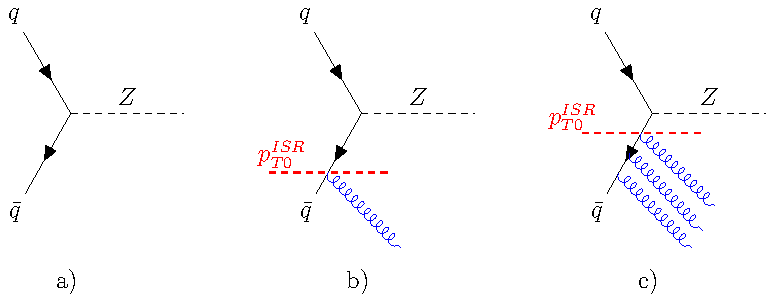
\includegraphics[width=0.8\textwidth]{{img/feynman_ZpT_2_blue.pdf}}
\end{figure}

With the addition of the primordial $k_T$ we get a Gaussian distribution that width is set by \texttt{BeamRemnants:primordialKThard}.
If we move to higher order diagrams the $Z$ boson can be produced with a non zero $p_T$, then the primordial $k_T$ is added. 

A large contribution come also from the amount of ISR that is emitted from the incoming partons, in fact each split can give to the incoming parton a non-zero initial value of $p_T$ and so the $Z$ boson is created with a non-zero $p_T$ before the introduction of the primordial $k_T$. 

An higher amount of ISR, so a lower value for the threshold, can lead to a larger $p_T$ taken from the parton that generate the $Z$ boson with an higher $p_T$ and vice versa.

\section{Primordial $k_T$ tune}

The primordial $k_T$ was not investigated by CP5 so it is important to include that in the analysis in order to describe better the low $p_T$ region. 

The parameters variation ranges we use are the one reported in the \tableRef{table:primordialkT_variations}. The other parameters are set to CP5 values.

\begin{table}[!htb]
\centering
\begin{tabular}{l | c }
Parameter Name & Value \\ 
\hline \hline
\\[-0.85em]
	\texttt{BeamRemnants:primordialKThard} & $[0.5 - 5.0]$\\[2pt]
	\texttt{SpaceShower:pT0Ref} & $[0.5 - 5.0]$\\
\end{tabular}
\caption{Variation ranges for the sampling used in the primordial $k_T$ tune.}
\label{table:primordialkT_variations}
\end{table} 

The number of samples is lower than the one used for the Underlying Event in fact the training set we use for the PerBin Model contains more or less $160$ MC runs and a little more for the Inverse Model, $\sim 200$.

To performed the tune the distribution used are from the \cite{ZpT_distributions} analysis at $\sqrt{s}=13\ \mathrm{TeV}$:
\begin{itemize}
	\item The $Z$ boson production cross-section in DY observation as a function of $p_T^Z$;
	\item The $Z$ boson production cross-section in DY observation as a function of $\phi_\eta^*$.
\end{itemize}

 
\begin{figure}[!htb]
	\centering
	\noindent
	\begin{subfigure}{0.48\textwidth}
	\centering
	\includegraphics[width=\textwidth]{{img/rivet-plots-PrimordialkT_PerBin_vs_Inverse_vs_CP5_FxFx_weights/CMS_2019_I1753680/d27-x01-y03.pdf}}	
	\end{subfigure}%
	\begin{subfigure}{0.48\textwidth}
	\centering
	\includegraphics[width=\textwidth]{{img/rivet-plots-PrimordialkT_PerBin_vs_Inverse_vs_CP5_FxFx_weights/CMS_2019_I1753680/d28-x01-y03.pdf}}	
	\end{subfigure}
\end{figure}

\begin{figure}[!htb]
	\centering
	\noindent
	\begin{subfigure}{0.48\textwidth}
	\centering
	\includegraphics[width=\textwidth]{{img/rivet-plots-PrimordialkT_PerBin_vs_Inverse_vs_CP5_FxFx_noWeights/CMS_2019_I1753680/d27-x01-y03.pdf}}	
	\end{subfigure}%
	\begin{subfigure}{0.48\textwidth}
	\centering
	\includegraphics[width=\textwidth]{{img/rivet-plots-PrimordialkT_PerBin_vs_Inverse_vs_CP5_FxFx_noWeights/CMS_2019_I1753680/d28-x01-y03.pdf}}	
	\end{subfigure}
\end{figure}


